\section{Experiments}
\label{sec:experiments}
\subsection{Setup}
We evaluate frozen CLIP ViT-B/32 experts~\cite{radford2021clip} on MNIST, SVHN, DTD, RESISC45, Cars, GTSRB, and SUN397. Complete test sets contain 10,000, 26,032, 1,880, 6,300, 8,041, 12,630, and 19,850 images, respectively. DTD uses the official test1 split. The eight-expert pool additionally contains EuroSAT; all reported task averages use the seven listed test sets.

Each two-expert experiment protects one expert and uses a fixed companion expert. MNIST uses SVHN as its companion; the other six use MNIST. Task Arithmetic uses coefficient 0.5 for each update. We compare unprotected experts, the official PaRaMS implementation with its fixed defaults, and \method. For AGA, the same author implementation processes the protected expert and the matching unprotected control before merging. It does not update the original expert through training.

Construction uses FP64 SVD with relative singular-value tolerance $10^{-10}$, a fixed random seed and the magnitude multiplier 2. Released parameters and inference use FP32. Every method uses the same checkpoints, classification heads and preprocessing. We report complete-test accuracy in percent, including companion-task accuracy. Among the procedures in \cref{tab:recovery}, only ProDistill uses training images. NBP construction uses none.

\subsection{Standalone utility and two-expert merging}
\Cref{tab:main} reports the seven protected tasks. After AGA and two-expert TA, mean target accuracy falls from 83.71\% to 3.29\% with \method{}. Five tasks retain every evaluated prediction. Cars has eight changed predictions and two net losses among 8,041 examples. SUN397 has four changed predictions and two net losses among 19,850 examples. The maximum standalone decrease is 0.025 percentage points.

Direct merging with PaRaMS or \method{} gives low target accuracy. AGA restores PaRaMS close to the unprotected control, while \method{} remains between 0.25\% and 9.80\%. AGA aligns attention and MLP parameters and leaves the final normalization bias fixed.

The loss of accuracy can be traced to a change in the prediction distribution. On MNIST, the protected AGA merge predicts digit 0 for all 10,000 examples (\cref{fig:predictions}), so its accuracy equals the test frequency of that digit, 9.80\%. The effect extends to the companion task: its mean accuracy across the seven pairs falls from 98.44\% to 15.72\% after AGA and TA (\cref{tab:partners}).

\begin{table}[!t]
\centering
\small
\setlength{\tabcolsep}{4pt}
\caption{Accuracy after AGA and TA across all 42 directed pairs (\%). Each row averages the six other validated tasks as companions. Subscripts t and c denote the protected target and companion; U is the unprotected control. The same seven NBP releases are used throughout.}
\label{tab:partners}
\begin{tabular}{lrrrr}
\toprule
Task & U$_t$ & NBP$_t$ & U$_c$ & NBP$_c$ \\
\midrule
SUN397 & 71.94 & 0.34 & 88.38 & 4.28 \\
Cars & 72.58 & 0.51 & 88.34 & 4.27 \\
RESISC45 & 91.19 & 2.44 & 84.26 & 8.17 \\
SVHN & 93.65 & 6.70 & 83.50 & 5.31 \\
GTSRB & 94.95 & 1.19 & 83.70 & 9.37 \\
MNIST & 99.30 & 9.80 & 82.12 & 2.80 \\
DTD & 70.07 & 2.13 & 88.52 & 5.86 \\
\bottomrule
\end{tabular}
\end{table}

\begin{figure}[!t]
\centering
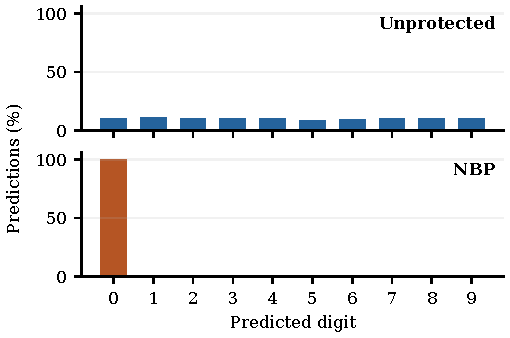
\includegraphics[width=\linewidth]{fig/predictions.pdf}
\caption{MNIST prediction frequencies after AGA and TA with the SVHN expert. The unprotected merge predicts all ten classes. With NBP, every example is assigned to digit 0.}
\label{fig:predictions}
\end{figure}

\subsection{Specified recovery procedures}
\begin{table}[!t]
\centering
\small
\setlength{\tabcolsep}{4pt}
\caption{Protected-task accuracy after the specified recovery procedures (\%). B reset replaces the final MLP output weight and bias after AGA, then applies TA. ProDistill uses its fixed layer-wise fitting protocol; final LayerNorm and projection are not optimized. The control receives the same processing.}
\label{tab:recovery}
\begin{tabular}{llrrr}
\toprule
Procedure & Defense & MNIST & SVHN & DTD \\
\midrule
\multirow{2}{*}{B reset} & None & 99.29 & 91.47 & 67.18 \\
 & \textbf{NBP} & 9.80 & 6.70 & 2.13 \\
\midrule
\multirow{3}{*}{ProDistill} & None & 99.45 & 96.73 & 73.14 \\
 & PaRaMS & 89.27 & 66.22 & 7.29 \\
 & \textbf{NBP} & 9.80 & 6.70 & 2.13 \\
\bottomrule
\end{tabular}
\end{table}

\paragraph{Public MLP replacement.}
Following the public-parameter replacement setting discussed in MergeBarrier~\cite{li2025mergebarrier}, our fixed check replaces the final MLP output matrix and its bias with the public base values. Replacement occurs after AGA and before TA. The operation is applied to both the protected model and the unprotected control. This is a native adaptation to the evaluated CLIP model, not a reproduction of the LLM experiment. Because it leaves the final LayerNorm bias unchanged, \method{} remains at 9.80\%, 6.70\%, and 2.13\% on MNIST, SVHN, and DTD.

\paragraph{Layer-wise coefficient fitting.}
We use the fixed author ProDistill kernel~\cite{xu2025prodistill}. The attacker has 64 unlabeled training images per task, task identity, and 100 coefficient-optimization steps per block, with initial coefficients 0.3. The two-expert adaptation updates element-wise block coefficients. The final LayerNorm and visual projection remain fixed throughout this procedure. The expert weights themselves are frozen. The unprotected and PaRaMS controls use the same data and fitting budget. The fits reduce PaRaMS accuracy on DTD as well as NBP accuracy, despite retaining 73.14\% in the unprotected control.

\subsection{Other fusion rules}
\begin{table}[!t]
\centering
\small
\setlength{\tabcolsep}{4pt}
\caption{Additional fusion rules on the fixed SUN397/MNIST pair (\%). TIES retains 20\% of entries with scale 1. DARE+TA uses drop rate 0.2, seed 42, and TA coefficient 0.5. AGA processes the protected expert. Both complete test sets and matching controls are reported.}
\label{tab:fusion}
\begin{tabular}{llrr}
\toprule
Fusion / recovery & Defense & SUN397 & MNIST \\
\midrule
\multirow{3}{*}{TIES} & None & 74.27 & 99.60 \\
 & PaRaMS & 0.29 & 8.92 \\
 & NBP & 0.25 & 10.28 \\
\midrule
\multirow{3}{*}{TIES + AGA} & None & 74.03 & 99.60 \\
 & PaRaMS & 74.03 & 99.60 \\
 & NBP & 0.25 & 10.28 \\
\midrule
\multirow{3}{*}{DARE+TA} & None & 71.87 & 99.45 \\
 & PaRaMS & 0.25 & 9.57 \\
 & NBP & 0.25 & 10.28 \\
\midrule
\multirow{3}{*}{DARE+TA + AGA} & None & 71.53 & 99.45 \\
 & PaRaMS & 71.53 & 99.45 \\
 & NBP & 0.25 & 10.28 \\
\bottomrule
\end{tabular}
\end{table}

\Cref{tab:fusion} evaluates the same frozen SUN397 releases with TIES and DARE+TA. TIES uses global top-20\% trimming and scale 1; DARE drops 20\% of task-update entries with fixed seed 42 before TA at 0.5. We use unchanged author kernels through the existing CLIP adapter. The settings are shared by all three defenses and are not selected from their test scores. With or without AGA, \method{} yields 50 correct SUN397 predictions out of 19,850, or 0.25\%. Companion MNIST accuracy is 10.28\%.

\subsection{Direction and magnitude}
\begin{table}[!t]
\centering
\small
\setlength{\tabcolsep}{4pt}
\caption{Direction controls on MNIST (\%). The three perturbations have the same update norm. The random nullspace direction is projected into the original visual-projection kernel; the unconstrained random direction uses the same sampled vector before projection. All controls use the same MNIST/SVHN pair and TA coefficient 0.5.}
\label{tab:ablation}
\begin{tabular}{lrrr}
\toprule
Update & Standalone & TA & AGA + TA \\
\midrule
None & 99.69 & 99.37 & 99.30 \\
NBP & 99.69 & 9.80 & 9.80 \\
Random nullspace & 99.69 & 65.21 & 63.74 \\
Random direction & 9.74 & 9.74 & 9.74 \\
\bottomrule
\end{tabular}
\end{table}

\Cref{tab:ablation} compares three perturbations of the same norm on MNIST. The random direction in the projection nullspace preserves standalone accuracy but gives 63.74\% after AGA and TA, compared with 9.80\% for NBP. The unconstrained random direction reduces standalone accuracy to 9.74\%. At this matched norm, the nullspace constraint preserves utility, while the class-directed solution causes a larger merged accuracy drop than the random nullspace control.

\begin{figure}[!t]
\centering
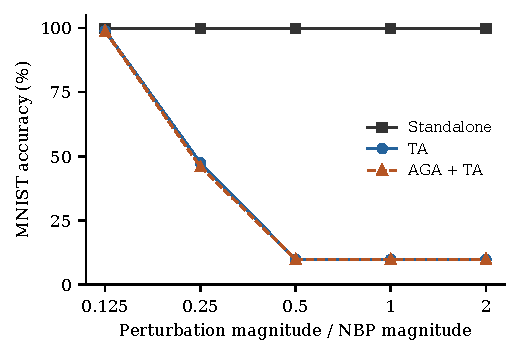
\includegraphics[width=\linewidth]{fig/amplitude.pdf}
\caption{Magnitude controls on the frozen MNIST perturbation, with SVHN as the companion. The horizontal axis rescales the published NBP update. Standalone accuracy is 99.69\% at all five magnitudes. Smaller updates at 0.125 and 0.25 retain substantial merged accuracy, while 0.5, 1, and 2 give 9.80\%. The released update corresponds to magnitude 1.}
\label{fig:amplitude}
\end{figure}
\Cref{fig:amplitude} varies only the update magnitude. At 0.125 of the NBP magnitude, MNIST accuracy after AGA and TA is 98.71\%; at 0.25 it is 45.88\%. The standalone predictions remain unchanged throughout the evaluated range.

\subsection{Multiple experts}
\Cref{tab:main} also reports eight-expert merging with TA coefficient 0.2, protecting one of the seven evaluated tasks at a time. All eight source experts participate in the author-specified order, including EuroSAT. After AGA, \method{} retains protected-task accuracies of 9.80\%, 6.70\%, and 2.13\% on MNIST, SVHN, and DTD, respectively; the corresponding scores are 2.44\%, 0.55\%, 1.19\%, and 0.25\% on RESISC45, Cars, GTSRB, and SUN397. AGA restores PaRaMS close to the matching unprotected result.

For each protected direction, we evaluate NBP and its unprotected control on all seven validated test sets. Thus the reported target-task entries are accompanied by a complete cross-task evaluation for these two methods. The coefficient $0.2$ multiplies each task update and gives the public base a coefficient of $1-8(0.2)=-0.6$ when written as a weighted sum of checkpoints.

\subsection{Fixed-readout analysis}
\begin{figure}[!t]
\centering
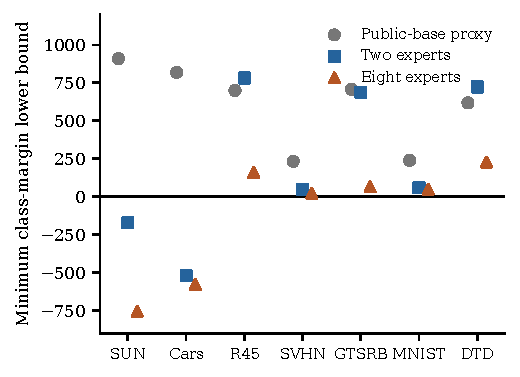
\includegraphics[width=\linewidth]{fig/readout_bound.pdf}
\caption{Minimum class-margin lower bound from \cref{eq:actualbound}, computed from the frozen NBP readout tensors. Positive values certify a constant prediction for every normalized hidden state in real arithmetic. Nonpositive values are inconclusive. SUN and R45 denote SUN397 and RESISC45. The public-base interpolation uses coefficient 0.5; actual two- and eight-expert TA use 0.5 and 0.2, respectively.}
\label{fig:readout}
\end{figure}
\Cref{fig:readout} examines seven frozen releases and their matching unprotected readouts in three settings, for 42 readouts in total. All seven protected public-base interpolations satisfy the bound. Five of seven actual two-expert models and five of seven actual eight-expert models also satisfy it. No matching unprotected model satisfies this sufficient condition. SUN397 and Cars do not satisfy it for the actual merges, despite their low measured accuracy; the sufficient bound does not describe every failure.

For the five certified tasks, modifying only earlier blocks cannot restore classification while keeping the stated readout fixed. This explains the measured failure of block-only alignment, final-MLP replacement, and the fixed ProDistill adaptation where applicable. It does not explain resistance to final-bias cleanup, which changes a parameter in the condition.

\subsection{A second vision backbone}
\begin{table}[!t]
\centering
\small
\setlength{\tabcolsep}{4pt}
\caption{CLIP ViT-B/16 protected-task accuracy (\%). The same NBP construction is applied to three experts. Two-expert TA uses coefficient 0.5; AGA processes the protected expert before merging.}
\label{tab:backbone}
\begin{tabular}{llrrr}
\toprule
Setting & Defense & MNIST & SVHN & DTD \\
\midrule
\multirow{2}{*}{Standalone} & None & 99.76 & 97.86 & 82.07 \\
 & \textbf{NBP} & 99.76 & 97.86 & 82.07 \\
\midrule
\multirow{2}{*}{TA} & None & 99.40 & 95.44 & 73.56 \\
 & \textbf{NBP} & 28.71 & 6.70 & 2.13 \\
\midrule
\multirow{2}{*}{AGA + TA} & None & 99.35 & 95.03 & 72.39 \\
 & \textbf{NBP} & 28.70 & 6.70 & 2.13 \\
\bottomrule
\end{tabular}
\end{table}

\Cref{tab:backbone} applies the same weight-only construction to CLIP ViT-B/16, whose final projection also has shape $768\times512$. All standalone predictions are preserved on the three full test sets. After AGA and TA, protected-task accuracy is 28.70\% on MNIST and 6.70\%/2.13\% on SVHN/DTD. Thus the effect transfers to this backbone, but MNIST does not reach the B/32 result. The AGA attention and MLP operations are unchanged and are applied to the B/16 architecture.

\subsection{Recovery at the final readout}
\label{sec:limitations}
\begin{table}[!t]
\centering
\small
\setlength{\tabcolsep}{4pt}
\caption{TA accuracy after public final-bias projection (\%). Columns give target (T) and companion (C) accuracy. Both releases receive the same cleanup before TA at 0.5. Their full prediction vectors are identical in these experiments.}
\label{tab:cleanup}
\begin{tabular}{lrrrr}
\toprule
Target & None T & None C & NBP T & NBP C \\
\midrule
MNIST & 99.37 & 92.50 & 99.37 & 92.50 \\
SVHN & 92.50 & 99.37 & 92.50 & 99.37 \\
DTD & 69.26 & 99.45 & 69.26 & 99.45 \\
\bottomrule
\end{tabular}
\end{table}

The preceding recovery procedures leave the final LayerNorm bias fixed. A method-specific attacker can instead remove its nullspace component using the published projection. For full-column-rank $P_e$, let $\Pi_e=P_e(P_e^{\mathsf T}P_e)^{-1}P_e^{\mathsf T}$. Then
\begin{equation}
 \begin{aligned}
 \Pi_e(b_e+\tau u)&=\Pi_e b_e,\\
 (\Pi_e b_e)^{\mathsf T}P_e&=b_e^{\mathsf T}P_e.
 \end{aligned}
 \label{eq:cleanup}
\end{equation}
This removes the added perturbation and preserves the standalone embedding, without data or the original expert. It need not recover the original bias itself. In the three-task experiment (\cref{tab:cleanup}), applying this operation to both NBP and its unprotected control gives identical merged predictions. No choice of magnitude or direction within the same kernel prevents this operation.

NBP therefore disrupts the evaluated merging and block-recovery procedures, but does not provide protection against arbitrary readout modification. Output calibration and student training in our additional recovery checks also restore accuracy. These outcomes distinguish the measured effect from a general white-box security claim.
